% $

\def \setA{ (0,0) circle (1cm) }
\def \setB{ (1.5,0) circle (1cm) }
\def \setC{ (60:1.5) circle (1cm) }
\def \setU{ (-2, -1.5) rectangle (3.5, 2.75) }
% \begin{center}
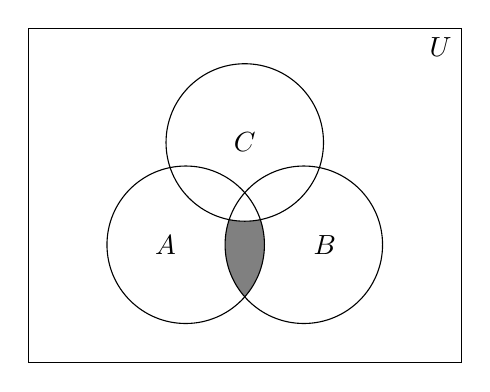
\begin{tikzpicture}
\draw \setU node[below left]{$U$};
        \begin{scope}
        \clip \setA;
        \fill[gray] \setB;
        \end{scope}
        \begin{scope}
        \clip \setA;
        \clip \setB;
        \fill[white] \setC;
        \end{scope}
\draw \setA node[left] {$A$}; \draw \setB node[right] {$B$}; \draw \setC node {$C$};
\end{tikzpicture}